\documentclass[screen,acmsmall]{acmart}
\settopmatter{printfolios=true,printccs=true,printacmref=true}

\bibliographystyle{ACM-Reference-Format}
\citestyle{acmauthoryear}   %% For author/year citations
\usepackage{mathpartir}
\usepackage[utf8]{inputenc}
\usepackage{fontenc}
\usepackage{microtype}
\usepackage{listings,array,multirow,wrapfig,xspace,booktabs,subcaption}
\usepackage{xcolor,tikz, graphicx, pifont}
\usetikzlibrary{positioning}

\newcommand{\authorcomment}[3]{\xspace\textcolor{#1}{{\bf #2} #3}\xspace} % start by defining an authorcomment

% For author notes:
%
\newcommand{\AG}[1]{\authorcomment{orange}{AG}{#1}}
\newcommand{\JV}[1]{\authorcomment{red}{JV}{#1}}
\newcommand{\JJ}[1]{\authorcomment{green}{JJ}{#1}}
\newcommand{\SK}[1]{\authorcomment{yellow}{SK}{#1}}

% For meta comments:
%
\newcommand{\isit}[1]{\authorcomment{cyan}{Check}{#1}}
\newcommand{\todo}[1]{\authorcomment{red}{TODO}{#1}}

\newcommand{\xmark}{\color{red} \ding{55}}
\newcommand{\cmark}{\color{green} \ding{51}}

\lstset{language=R}

\definecolor{LightGray}{rgb}{.92,.92,.92}
\definecolor{Gray}{rgb}{.3,.3,.3}
\definecolor{DarkGray}{rgb}{.5,.5,.5}

\lstset{ %
  columns=flexible,
  captionpos=b,
  frame=single,
  framerule=0pt,
  framexleftmargin=-1mm,
  framexrightmargin=-1mm,
  tabsize=2,
  belowskip=0pt,
  basicstyle=\small\ttfamily,
  backgroundcolor=\color{LightGray},
  emphstyle=\sffamily,
  keywordstyle=\bfseries,
  commentstyle=\color{Gray}\em,
  stringstyle=\color{Gray}
}
\lstdefinestyle{R}{ %
  language=R,
  deletekeywords={new, env, equal, c, runif, trace, args, exp, t, all, get,
    names, is, environment, class, substitute, expression, list, null, Internal,
    sample, diag, length, rep, nrow, stop, offset, pmax, Machine,
    double, parent, frame, par, methods, end, dir, apply, deparse, missing,
    plot, as, integer, character, inherits, numeric, paste, eval, quote, call,
    formula, df, log, sum, c, local, legend, file, scale, round, title, order,
    drop, which, grid, print, ncol, dim, max, format, sort, rug, matrix, start,
    unique, mean, df, attr, do, power},
  otherkeywords={},
  breaklines=true
}

\newcommand{\code}[1]{\lstinline[style=R]|#1|\xspace}
\renewcommand{\c}[1]{\lstinline[style=R]|#1|\xspace}
\newcommand{\lazr}{\emph{lazr}}
\newcommand{\strictr}{\emph{strictr}}
%%% \setcopyright{rightsretained}
%%% \acmPrice{}
%%% \acmDOI{10.1145/3360579}
%%% \acmYear{2019}
%%% \copyrightyear{2019}
%%% \acmJournal{PACMPL}
%%% \acmVolume{3}
%%% \acmNumber{OOPSLA}
%%% \acmArticle{153}
%%% \acmMonth{10}
\begin{document}
\title{Promises are made to be broken}
\subtitle{On providing strict evaluation semantics for the R language}

\author{Aviral Goel}\affiliation{\institution{Northeastern University}\country{USA}}
\author{Jan Ječmen}\affiliation{\institution{Czech Technical University}\country{Czechia}}
\author{Sebastián Krynski}\affiliation{\institution{Czech Technical University}\country{Czechia}}
\author{Oliver Flückiger}\affiliation{\institution{Northeastern University}\country{USA}}
\author{Jan Vitek}\affiliation{\institution{Czech Technical University and Northeastern University}\country{USA}}
\authorsaddresses{}
\renewcommand{\shortauthors}{Goel, Vitek}

\begin{abstract}
  Function calls in the R language do not evaluate their arguments, these are
  passed as suspended computations to the callee which will evaluate them only
  if they are needed. After 25 years of experience with the language, there are
  very few cases where delayed evaluation is being intentionally leveraged by
  programmers. Yet being lazy comes at a price in performance and complexity.
  This paper explores what would happen if the semantics of the language was
  changed to become strict-by-default and lazy-on-demand. To answer this
  question we implemented a dynamic analysis that synthesizes strictness
  signatures for functions. Given such signature, we implemented a tool that
  automatically transforms source code to enforce the signatures. We then
  performed a large scale evaluation of the robustness of the inferred
  signature. Finally we explored the impact of providing strictness signatures
  on a just-in-time compiler.
\end{abstract}

\begin{CCSXML}
<ccs2012>
<concept>
<concept_id>10002944.10011123.10010912</concept_id>
<concept_desc>General and reference~Empirical studies</concept_desc>
<concept_significance>500</concept_significance>
</concept>
<concept>
<concept_id>10011007.10011006.10011008</concept_id>
<concept_desc>Software and its engineering~General programming languages</concept_desc>
<concept_significance>500</concept_significance>
</concept>
<concept>
<concept_id>10011007.10011006.10011050.10010517</concept_id>
<concept_desc>Software and its engineering~Scripting languages</concept_desc>
<concept_significance>500</concept_significance>
</concept>
<concept>
<concept_id>10011007.10011006.10011039.10011311</concept_id>
<concept_desc>Software and its engineering~Semantics</concept_desc>
<concept_significance>300</concept_significance>
</concept>
</ccs2012>
\end{CCSXML}

\ccsdesc[500]{General and reference~Empirical studies}
\ccsdesc[500]{Software and its engineering~General programming languages}
\ccsdesc[500]{Software and its engineering~Scripting languages}
\ccsdesc[300]{Software and its engineering~Semantics}

\keywords{R language, delayed or lazy evaluation}

\maketitle
\section{Introduction}

The R programming language is widely used in data science. Unbeknownst to many
of its end-users, function calls have a call-by-need, or lazy, semantics. In
other words the arguments of a function call are suspended computations which
are evaluated if and when they are needed. \citet{oopsla19b} provided a thorough
observational study of a corpus consisting of 16,707 packages written in R. For
the most part, the corpus appears to have been written without reliance on
laziness with the exception of code that leverages it for meta-programming.

This paper argues that laziness should be the exception in R. We propose to make
it a \emph{eager by default, lazy on demand} language by introducing strictness
annotations. The question we wish to answer is whether it is possible to switch
the semantics of a language without causing undue breakage in the legacy code
that is in daily use. This concern is relevant because, even if programmers
don't avail themselves of call-by-need, it is conceivable that their code
accidentally depends on it. A change in the order of evaluation of arguments may
introduce errors if that code was performing side effects.

\paragraph{The Case for Strictness.} Laziness is error-prone, inconsistent
and costly. The combination of delayed evaluation and side-effects in a language
without type annotations is an invitation to subtle programming errors. If a
function has multiple evaluation orders and is called with effectful arguments,
their effects will be observed to happen in various orders. Functional languages
prevent ordering issues by reflecting effects in the type system. R cannot do
this as it is dynamically typed. Instead, libraries routinely add code at the
boundaries of their API to force a single evaluation order. The design and use
of call-by-need is inconsistent because there are multiple points where
evaluation is arbitrarily forced. These include right-hand side of assignments
and function returns, neither of which is required in a lazy language.
Furthermore, to support object-oriented programming, R allows both single- and
multiple-dispatch; in order to perform dispatch, arguments must be evaluated
eagerly. Last, there are costs to lazy evaluation. Each argument must be boxed
in a data structure that holds a reference to the expression to evaluate, its
environment and the result of evaluation. Allocating and deallocating these data
structures put pressure on the memory manager. Delayed evaluation further
complicates the work of compilers for the language by hindering optimizations
and increasing the number of indirect calls.

\paragraph{The Case for Laziness.} The success of a programming language
often comes down to the strength of its ecosystem. With tens of millions of
lines of contributed library code, any change to the core semantics of the
language risks changing the behavior of some library functions. Preserving the
status quo is a pragmatic choice to protect the investment in legacy code bases.
Laziness is needed for an additional reason, it is the building block of the
meta-programming facilities of the language. Unevaluated arguments can be
coerced back to their source code, that code can be modified, and evaluated in
an environment of the programmer's choice. Meta-programming is used to extend
the language and to create embedded domain specific languages. While it is
possible to imagine using macros instead, the number of libraries that use
meta-programming is sufficiently large that it would be non-trivial to refactor
them.

\section{Background}
\subsection{The R Language}

\subsection{Missingness}

A function in R can be called with fewer arguments than expected. These
argumentless parameters are treated as missing if they don't have a default
value. The function can check for missing arguments using the \code{missing}
function. Since missing arguments can be forwarded to callees, \code{missing}
performs this check transitively. The strictness signatures we compute reflect
the function's strictness with respect to its arguments when they are not
missing.


\subsection{Metaprogramming}
The \code{substitute} function provides reflective access to an argument's
unevaluted code contained inside the promise. This can also be done in native
code using the \code{PREXPR} C macro on the promise object. These cases reflect a
genuine use of laziness. Functions are treated as lazy in these arguments, even
if the arguments are evaluated.

\subsection{Reflection}
R provides reflective access to its first class environments and it 

\subsection{Effects}

\subsection{Vararg}
varargs, or $...$ paramaters, accept an arbitrary number of arguments, including
missing arguments. The function can materialize $...$ into a list using the
\code{list(...)} pattern. This saves the user from packaging the arguments into
a list. The function can also forward its $...$ to a callee. This enables the
function to expose its callee's interface to the callers without listing
callee's parameters and their default values. 




\subsection{Related Work}
The foundation for our work is \cite{oopsla19b}'s work on the design,
implementation, and use of laziness in R. They provide a detailed account of R's
call-by-need evaluation strategy with a small-step operational semantics and an
empirical evaluation of 16,707 R packages. Their study shows that R is rather
strict for a lazy language, with most R code written without reliance on
laziness. In their corpus of 388.3K functions, they identify 83.7\% functions as
strict, i.e., these functions evaluate all of their arguments in a single order
across all calls. The authors find that R programmers ``force'' arguments at the
beginning of a function for a deterministic evaluation order. The authors
identify only one instance of lazy data structure and find that meta-programming
is the only dominant use of R's laziness.

\cite{oopsla20b}'s work on empirically inferring type signatures for R functions
is very similar to our work in spirit. They synthesize function type signatures
by dynamically observing the type of function arguments and return values. They
validate these signatures by inserting type checking code inside functions and
monitor type contract failure by running client programs. Failed type contracts
can be detected at a function's boundary by comparing a value's actual type
against its expected type. However, evaluating an argument on function entry
does not prohibit it from being used in a non-strict setting such as
metaprogramming. A side-effecting argument which would otherwise not have been
evaluated by the function could still be evaluated according to our strictness
signature without an observable error. This makes validation of strictness
signatures hard.

With this work, we are trying to propose a change in the semantics of R. There
are many other instances of mainstream languages incorporating a major change in
semantics. The most prominent example is the transition from Python 2 to Python
3, which is still an ongoing process. Python 3 was released in 2008 with a
plan\cite{pysunset} to drop support for Python 2 in 2015. This was later
extended to 2020 since a lot of codebase in 2015 was not transitioned to Python
3. However, legcay codebase continues to run on Python 2 till date. Python 3
introduced many incompatible changes without any tooling support for transition.
py2to3 script only handles a selection of superficial changes. TODO.

TODO: Autobahn (haskell strictness signature).

Similar to our attempts to modify R's semantics are the transition from Python 2
to Python 3, PHP to Hack, introduction of Javascript's strict mode and 

\section{Strictness Signatures}

A function's strictness signature is a tuple $\langle f, s_1, ..., s_n \rangle$,
where $f$ is the function's qualified name and $s_i$ are positions of arguments
that can be evaluted strictly. We synthesize these signatures from dynamically
generated traces. The decision to make a function strict in a particular
argument is conditioned on the aspects discussed below.

Arguments used for metaprogramming using \code{substitute} and \code{PREXPR} are
never strict. These argument promises cannot be eliminated without breaking
code.

$...$ arguments are always treated as lazy. Assigning a single strictness
annotation to $...$ is tricky because a function can have different strictness
behavior for the individual arguments of $...$. One solution is to treat the
function strict in $...$, if it is strict in all of its constituents. However,
assigning a unique strictness signature to $...$ is difficult because a function
may itself use them in a strict setting but its callees may use metaprogramming
on the promises inside $...$. This is possible because unlike normal argument
promises, promises inside $...$ are not packaged in a new promise but rather
forwarded as-is to callees. Furthermore, a $...$ passed to a callee could be
forwarded further down resulting in a long chain of functions having access to
the same argument promises. All these functions in the chain can directly affect
these arguments. The presence of missing arguments inside $...$ introduces
another wrinkle.

Functions \code{as.environment} and \code{pos.to.env} when invoked with argument
\code{-1} return the environment of the current call on the stack. Calling them
directly from inside a promise makes the promise's result sensitive to the frame
of its evaluation. This makes the function lazy in that argument even if its
implementation does not require this argument to be lazy. This code has an
accidental reliance on laziness. If the function's documentation does not make
any commitment about the frame in which this argument will be evaluated, this
code will be susceptible to breakage due to change in the function's
implementation.

Arguments can perform side-effects. Many argument promises will contain a symbol
referring to the value being passed as the argument, so they will at least
perform a read in the caller's environment. Similarly, some promises contain
function call expressions which will do local writes in the environment created
for the function call during promise evaluation. These effects are benign and do
not affect our decision to evaluate the corresponding arguments strictly.
However, if a promise writes to the caller's environment, or more generally, to
any environment that is not created during its evaluation, then that write is
observable by code outside the promise. Also, if a promise reads from an
environment that is modified after the promise is created and before it is
evaluated, then that argument can also be treated lazily. Arguments that perform
these reads and writes depend on the evaluation order implemented by the
function to which they are passed. Unless the function's documentation describes
this order, these uses are wrong. A change in function's implementation could
cause the reads and writes to happen in a different order, or not at all,
leading to incorrect results.

Errors are another source of effect inside promises. They can either stop the
program execution or captured by an enclosing exception handler. Just like
TODO.


Finally, if an argument is not evaluated in all calls to the function, the
function is not strict in that argument. We could still evaluate the argument.
Unless the documentation dictates that this argument is evaluated in special
cases where it could be reflective or side-effecting, we could still evaluated
it without any observable consequence except a performance penalty.


In summary, $...$ and arguments that are metaprogrammed are always lazy. In
contrast to side-effecting and reflective promises these are genuine uses of
laziness as they are not affected by the client. To get rid of promises
aggressively, We could try evaluating the arguments it strictly, but it could either throw an
error, perform a side-effect, or just affect performance.







for
\emph{(a)} to forward the arguments to a callee \emph{(b)} to number of
arguments for strictness signatures. strict. ... effect as.environment

Firstly, 
The first source of laziness is when an argument is not
used in a call to the function. Such arguments could still be evaluated strictly
but there might be a significant performance penalty, or worse, a side-effect.
Even reads performed by the argument could trigger evaluation of promises that
could lead to side-effects.

There are 2 internal sources of
laziness in R: metaprogramming, and unused arguments.

A combination of these choices results in many
possible signature configurations.





\subsection{Synthesizing Signatures}

\section{Analysis Infrastructure}
In this section, we describe the analysis pipeline that \emph{(a)} profiles R
programs for laziness, \emph{(b)} extracts and analyzes strictness signatures
from the profile, and \emph{(c)} validates those signatures by eagerly forcing
function arguments. The analysis pipeline starts with setting up a Docker image
that includes all the dependencies for installing analysis code and R packages
from CRAN and Bioconductor. This provides a reliable reproducible setup across
the three machines. Next, we mirror CRAN and Bioconductor\cite{bioc} repositories and
install their R packages. This is followed by generation of execution traces
from a dynamic analyzer running inside an instrumented R virtual machine. These
traces are analyzed to generate tabular data files and strictness signatures.
Finally, the signatures are applied to client programs for validation. Our
experiments were performed on three Intel Xeon 6140, 2.30GHz machines with 72
cores and 256GB of RAM each. The pipeline is managed by a Makefile which has
rules for every step. This makes it easy to administer the experiments on
multiple machines. Whenever possible, we parallelize the steps using GNU
parallel\cite{tange2011a}.

\subsection{Synthesizing Strictness Signatures}

A function's strictness signature is a tuple $\langle f, s_1, ..., s_n
\rangle$, where $f$ is the function's qualified name and $s_i$ are positions of arguments that can be
evaluted strictly. We synthesize these strictness signatures for functions by
observing the evaluation of their arguments at runtime. For this, we use three
tools that enable us to dynamically inspect a function call's arguments.

%% R-dyntrace

First,
we use an instrumented R virtual machine, \emph{R-dyntrace} \citet{oopsla19b}
based on GNU-R version 4.0.2. The framework provides an event framework for
invoking user-defined callbacks at specific points inside the R interpreter.
\emph{R-dyntrace} supplies raw R objects to the callbacks. Extracting meaningful
information at this low level requires handling a lot of subtleties arising from
the intricacies of R's implementation and execution model. These details are
surprisingly hard to get right, even for simple progrms. The challenges are
described in detail by \cite{oopsla19b} in the design of their tracer for
collecting information about use of laziness in R programs.

%% instrumentr

To iron these wrinkles, we developed \emph{instrumentr}, an R package that
provides a layer of abstraction on top of the event framework exposed by
\emph{R-dyntrace}. \emph{instrumentr} provides API to create tracer objects to
which event specific callbacks can be attached. \emph{instrumentr} intercepts
\emph{R-dyntrace} events and invokes the corresponding tracer's callbacks. It
passes model objects to callbacks by wrapping the raw R objects provided to
its own callbacks registered with \emph{R-dyntrace}.
\begin{itemize}
\item These model objects contain metadata about the raw R object and provide a
  consistent API for inspecting their constituents.
\item The object metadata keeps track of the object's unique id. This uniqueness
  guarantee enables downstream client analyses to key objects by their id
  instead of addresses which are not unique since they get resused by R's
  garbage collector.
\item The model objects are reference counted which makes it possible for a
  model object to be referenced by multiple model objects with proper memory
  management. A complication arises in this design when objects have cyclic
  references. For example, a promise argument keeps a reference to a call object
  and vice-versa. To address this, \emph{instrumentr} defines the notion of a
  primary owner. The primary owner of a model object can ``kill'' the object,
  i.e. free up object's internals (and decrement the references it holds to
  other objects) even if it is referenced by other objects. Killing does not
  free up the model object's memory or affect its metadata. This lets secondary
  owners access the dead object's metadata even after the raw R object no longer
  exists. The ``dead'' object's memory is finally freed when it is no longer
  referenced by any other object in the system. This design insight makes it
  trivial to express complex object dependencies without any memory leaks at the
  scale of millions of objects. This also enables clients to query dead object's
  metadata if they are referenced by model objects made available to the clients
  via their callbacks. This greatly simplifies the handling of promises, first
  class environments and function calls.
\item \emph{instrumentr} keeps track of logical time, from tracing entry to
tracing exit, incremented on every event. The model object's metadata keeps
track of its time of allocation and deallocation. For environments, it also
keeps track of last read and last write time. For promises, it keeps track of
force entry and force exit time. This information is used to identify non-local
reads and writes to environments. The model objects are cached in a table keyed
by the R object's address. Table entries are inserted and erased on \emph{object
  allocation and deallocation} events respectively. This prevents duplication of
model objects when the same R object is encountered on multiple events.
\item \emph{instrumentr} models the call stack. It also adds promise objects under
evaluation to the stack. This helps identify if an event, say a side-effect, is
occuring inside a promise. Furthermore, R uses \emph{longjmp} to do non-local
returns. \emph{instrumentr} exposes a deterministic behavior during such events
by artificially calling the exit callbacks of interrupted calls and promises on
the stack. This simplifies the client side tracing logic, significantly.
\item \emph{instrumentr} keeps track of environment and function names in their model
objects. Getting fully qualified function names dynamically is challenging in R
becausse packages are first class environments that are constructed piecemeal
and all functions are by default anonymous objects that may be bound to a name
in their lexical scope. \emph{instrumentr} handles this by assigning names to
environments on package load events and checking on every write if a function is
being bound to a name. Functions can be nested to arbitrary depths in which case
\emph{instrumentr} links model function objects to reflect the parent-child
relationship.
\end{itemize}
%% lazr

For extracting execution
traces, we developed \emph{lazr}, an R library which sits atop
\emph{instrumentr}. \emph{lazr} collects information about function calls,
arguments, side-effects, and reflective environment access. from the model
objects provided by the following instrumentr event: \emph{function entry and
  exit}, \emph{promise evaluation entry and exit}, \emph{variable reads and
  writes}, \emph{promise value and expression reads}, and \emph{function
  lookup}. This information is stored in compressed tabular format using R's
\emph{fst} library. Analysis scripts provided by \emph{lazr} use this data to
synthesize strictness signatures.

zoo::merge.zoo redefines f with different number of parameters.

\subsection{Applying Strictness Signatures}

To apply a function's strictness signature, we force the corresponding
arguments on every call to that fuction. For this, we developed \emph{strictr},
an R package that adds code to force arguments at the top of a function's
definition. R allows packages to register callbacks which are invoked when a
package is loaded by the program. \emph{strictr} sets up a package load callback
for all the packages for which we generate signatures. When a program loads a
package, \emph{strictr}'s callback is invoked. \emph{strictr} reads the
signatures for functions of the loaded package from a file, and injects code in
the function's definition in accordance with the signature. The injected code
first checks for missingness and evaluates the argument only if it is supplied
by the user or has a default value. The arguments are evaluated in the order
specified by the signature. \emph{strictr} also supports nested functions by
recursively descending into the parent function's definitions until it finds the
inner function binding. Signatures are made available to \emph{strictr} as a
directory containing one file per package. Providing signatures in external
files avoids the need to modify the source code of programs. This also enables
easy experimentation with different signature configurations by providing a
different directory location.

Talk about  \code{is_same_body <<- is_reference}

%%% TODO:
%%% \begin{lstlisting}[language=R]
%%% 
%%% 
%%% 
%%% \end{lstlisting}

\section{Corpus of R Programs}

For synthesizing strictness signatures, we run code from a corpus of packages
using \lazr. For validation, we insert strictness contracts in the corpus
functions and run their client programs using \strictr.

We selected corpus packages and client programs from CRAN and Bioconductor, two
official package repositories for R. CRAN and Bioconductor have 17,388 and 3,344
packages each, of which, we were able to install 17,142 CRAN and 2,733
Bioconductor packages. Some packages could not be installed because of missing
native dependencies and compilation errors in our Docker image. We chose to
discard those packages. Code submitted to CRAN and Bioconductor is curated by
subjecting it to a battery of tests to ensure quality. Packages submitted to
these repositories have runnable code in the form of tests, examples, and
vignettes. Vignettes are typically long examples which demonstrate a packages
functionality.

We synthesized signatures for functions from 500 packages. The criterion was to
select packages with the maximum number of client packages. This requirement
enabled us to evaluate the strictness signatures of those packages from the
runnable code of their clients. The chosen packages have a total of 15,362
dependent client packages, ranging from maximum 2,669 dependents for
\emph{ggplot2} to minimum 5 for \emph{spatstat.linnet} with an average 125.4
dependents.

The selected 500 packages have 2.2M lines of R code and 2.7M lines of native (C,
C++, and Fortran) code. For synthesizing signatures for their functions, we
analyzed the execution traces obtained from their examples, tests, and
vignettes.

\begin{wraptable}{r}{7cm}
  \vspace{-3mm}
  \small
  \caption{Corpus}\label{table:corpus}
  \vspace{-3mm}
  \begin{tabular}{l|rrrl} %{@{}l|r@{~~}r@{~}r@{~~}l@{}}
    &\bf Tests&\bf Examples&\bf Vignettes&\\\hline
    \multirow{2}{*}
    {Scripts}&5.8K&20.2K&631&\it Corpus\\
    &9.8K&41.1K&1.7K&\it Client\\\hline
    \multirow{2}{*}
    {LOC}&406.4K&207.0K&48.7K&\it Corpus \\
    &751.2K&348.8K&112.3K&\it Client \\\hline
  \end{tabular}
\end{wraptable}

For validation, we selected 2000 dependent packages of the synthesis
corpus. They have 4.5M lines of R code and 4.7M lines of native (C, C++, and
Fortran) code. We run their examples, tests, and vignettes to exercise the
functions with signatures.

Table ~\ref{table:corpus} gives the number of scripts of each kind that were run
and lines of code exercised.

\begin{wraptable}{l}{8cm}
  \vspace{-3mm}
  \small
  \caption{Package Size} \label{table:packsize}
  \centering
  \begin{tabular}{lr}
    \bf Functions&\bf Packages\\
    \hline
    1--25&148\\
    26--50&98\\
    51--75&52\\
    76--100&33\\
    101--150&54\\
    151--200&34\\
    201--250&28\\
    \hline
  \end{tabular}
  \quad
  \begin{tabular}{lr}
    \bf Functions&\bf Packages\\
    \hline
    251--300&16\\
    301--400&14\\
    401--500&7\\
    501--600&5\\
    601--700&1\\
    701--800&4\\
    801--900&2\\
    \hline
  \end{tabular}
\end{wraptable}

We generate signatures for 50,435 functions from 500 packages. These are
top-level package functions. We ignore anonymous and inner functions. Table
~\ref{table:packsize} shows the distribution of these functions across packages.
We observe that 148 packages have 25 functions or less. As expected, there is a
steady decrease in packages with more functions. There are 12 packages with more
than 500 functions. Package \emph{spatstat.geom} has the maximum number of
functions, 886.

\begin{figure}[!h]
  \centering
  % Created by tikzDevice version 0.12.3.1 on 2021-04-09 21:52:41
% !TEX encoding = UTF-8 Unicode
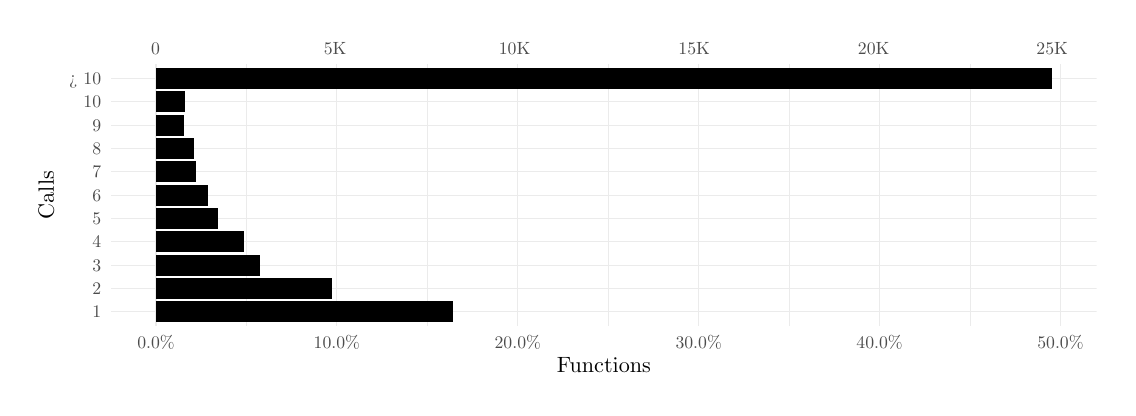
\begin{tikzpicture}[x=1pt,y=1pt]
\definecolor{fillColor}{RGB}{255,255,255}
\path[use as bounding box,fill=fillColor,fill opacity=0.00] (0,0) rectangle (390.26,130.09);
\begin{scope}
\path[clip] ( 30.17, 22.32) rectangle (386.26,116.83);
\definecolor{drawColor}{gray}{0.92}

\path[draw=drawColor,line width= 0.2pt,line join=round] ( 79.04, 22.32) --
	( 79.04,116.83);

\path[draw=drawColor,line width= 0.2pt,line join=round] (144.41, 22.32) --
	(144.41,116.83);

\path[draw=drawColor,line width= 0.2pt,line join=round] (209.77, 22.32) --
	(209.77,116.83);

\path[draw=drawColor,line width= 0.2pt,line join=round] (275.14, 22.32) --
	(275.14,116.83);

\path[draw=drawColor,line width= 0.2pt,line join=round] (340.51, 22.32) --
	(340.51,116.83);

\path[draw=drawColor,line width= 0.4pt,line join=round] ( 30.17, 27.38) --
	(386.26, 27.38);

\path[draw=drawColor,line width= 0.4pt,line join=round] ( 30.17, 35.82) --
	(386.26, 35.82);

\path[draw=drawColor,line width= 0.4pt,line join=round] ( 30.17, 44.26) --
	(386.26, 44.26);

\path[draw=drawColor,line width= 0.4pt,line join=round] ( 30.17, 52.70) --
	(386.26, 52.70);

\path[draw=drawColor,line width= 0.4pt,line join=round] ( 30.17, 61.14) --
	(386.26, 61.14);

\path[draw=drawColor,line width= 0.4pt,line join=round] ( 30.17, 69.58) --
	(386.26, 69.58);

\path[draw=drawColor,line width= 0.4pt,line join=round] ( 30.17, 78.01) --
	(386.26, 78.01);

\path[draw=drawColor,line width= 0.4pt,line join=round] ( 30.17, 86.45) --
	(386.26, 86.45);

\path[draw=drawColor,line width= 0.4pt,line join=round] ( 30.17, 94.89) --
	(386.26, 94.89);

\path[draw=drawColor,line width= 0.4pt,line join=round] ( 30.17,103.33) --
	(386.26,103.33);

\path[draw=drawColor,line width= 0.4pt,line join=round] ( 30.17,111.77) --
	(386.26,111.77);

\path[draw=drawColor,line width= 0.4pt,line join=round] ( 46.36, 22.32) --
	( 46.36,116.83);

\path[draw=drawColor,line width= 0.4pt,line join=round] (111.72, 22.32) --
	(111.72,116.83);

\path[draw=drawColor,line width= 0.4pt,line join=round] (177.09, 22.32) --
	(177.09,116.83);

\path[draw=drawColor,line width= 0.4pt,line join=round] (242.46, 22.32) --
	(242.46,116.83);

\path[draw=drawColor,line width= 0.4pt,line join=round] (307.82, 22.32) --
	(307.82,116.83);

\path[draw=drawColor,line width= 0.4pt,line join=round] (373.19, 22.32) --
	(373.19,116.83);
\definecolor{fillColor}{RGB}{0,0,0}

\path[fill=fillColor] ( 46.36,107.97) rectangle (370.07,115.57);

\path[fill=fillColor] ( 46.36, 23.58) rectangle (153.52, 31.18);

\path[fill=fillColor] ( 46.36, 99.53) rectangle ( 56.78,107.13);

\path[fill=fillColor] ( 46.36, 32.02) rectangle (109.88, 39.62);

\path[fill=fillColor] ( 46.36, 40.46) rectangle ( 83.98, 48.06);

\path[fill=fillColor] ( 46.36, 48.90) rectangle ( 78.12, 56.49);

\path[fill=fillColor] ( 46.36, 57.34) rectangle ( 68.81, 64.93);

\path[fill=fillColor] ( 46.36, 65.78) rectangle ( 65.03, 73.37);

\path[fill=fillColor] ( 46.36, 74.22) rectangle ( 60.74, 81.81);

\path[fill=fillColor] ( 46.36, 82.66) rectangle ( 60.20, 90.25);

\path[fill=fillColor] ( 46.36, 91.10) rectangle ( 56.47, 98.69);
\end{scope}
\begin{scope}
\path[clip] (  0.00,  0.00) rectangle (390.26,130.09);
\definecolor{drawColor}{gray}{0.30}

\node[text=drawColor,anchor=base,inner sep=0pt, outer sep=0pt, scale=  0.64] at ( 46.21,120.43) {0};

\node[text=drawColor,anchor=base,inner sep=0pt, outer sep=0pt, scale=  0.64] at (111.09,120.43) {5K};

\node[text=drawColor,anchor=base,inner sep=0pt, outer sep=0pt, scale=  0.64] at (175.96,120.43) {10K};

\node[text=drawColor,anchor=base,inner sep=0pt, outer sep=0pt, scale=  0.64] at (240.83,120.43) {15K};

\node[text=drawColor,anchor=base,inner sep=0pt, outer sep=0pt, scale=  0.64] at (305.70,120.43) {20K};

\node[text=drawColor,anchor=base,inner sep=0pt, outer sep=0pt, scale=  0.64] at (370.22,120.43) {25K};
\end{scope}
\begin{scope}
\path[clip] (  0.00,  0.00) rectangle (390.26,130.09);
\definecolor{drawColor}{gray}{0.30}

\node[text=drawColor,anchor=base east,inner sep=0pt, outer sep=0pt, scale=  0.64] at ( 26.57, 25.18) {1};

\node[text=drawColor,anchor=base east,inner sep=0pt, outer sep=0pt, scale=  0.64] at ( 26.57, 33.62) {2};

\node[text=drawColor,anchor=base east,inner sep=0pt, outer sep=0pt, scale=  0.64] at ( 26.57, 42.05) {3};

\node[text=drawColor,anchor=base east,inner sep=0pt, outer sep=0pt, scale=  0.64] at ( 26.57, 50.49) {4};

\node[text=drawColor,anchor=base east,inner sep=0pt, outer sep=0pt, scale=  0.64] at ( 26.57, 58.93) {5};

\node[text=drawColor,anchor=base east,inner sep=0pt, outer sep=0pt, scale=  0.64] at ( 26.57, 67.37) {6};

\node[text=drawColor,anchor=base east,inner sep=0pt, outer sep=0pt, scale=  0.64] at ( 26.57, 75.81) {7};

\node[text=drawColor,anchor=base east,inner sep=0pt, outer sep=0pt, scale=  0.64] at ( 26.57, 84.25) {8};

\node[text=drawColor,anchor=base east,inner sep=0pt, outer sep=0pt, scale=  0.64] at ( 26.57, 92.69) {9};

\node[text=drawColor,anchor=base east,inner sep=0pt, outer sep=0pt, scale=  0.64] at ( 26.57,101.13) {10};

\node[text=drawColor,anchor=base east,inner sep=0pt, outer sep=0pt, scale=  0.64] at ( 26.57,109.57) {> 10};
\end{scope}
\begin{scope}
\path[clip] (  0.00,  0.00) rectangle (390.26,130.09);
\definecolor{drawColor}{gray}{0.30}

\node[text=drawColor,anchor=base,inner sep=0pt, outer sep=0pt, scale=  0.64] at ( 46.36, 14.31) {0.0{\%}};

\node[text=drawColor,anchor=base,inner sep=0pt, outer sep=0pt, scale=  0.64] at (111.72, 14.31) {10.0{\%}};

\node[text=drawColor,anchor=base,inner sep=0pt, outer sep=0pt, scale=  0.64] at (177.09, 14.31) {20.0{\%}};

\node[text=drawColor,anchor=base,inner sep=0pt, outer sep=0pt, scale=  0.64] at (242.46, 14.31) {30.0{\%}};

\node[text=drawColor,anchor=base,inner sep=0pt, outer sep=0pt, scale=  0.64] at (307.82, 14.31) {40.0{\%}};

\node[text=drawColor,anchor=base,inner sep=0pt, outer sep=0pt, scale=  0.64] at (373.19, 14.31) {50.0{\%}};
\end{scope}
\begin{scope}
\path[clip] (  0.00,  0.00) rectangle (390.26,130.09);
\definecolor{drawColor}{RGB}{0,0,0}

\node[text=drawColor,anchor=base,inner sep=0pt, outer sep=0pt, scale=  0.80] at (208.22,  5.56) {Functions};
\end{scope}
\begin{scope}
\path[clip] (  0.00,  0.00) rectangle (390.26,130.09);
\definecolor{drawColor}{RGB}{0,0,0}

\node[text=drawColor,rotate= 90.00,anchor=base,inner sep=0pt, outer sep=0pt, scale=  0.80] at (  9.51, 69.58) {Calls};
\end{scope}
\end{tikzpicture}

  \caption{Call Distribution}
  \label{fig:callDist}
\end{figure}

We observe 137.2M calls to these functions. Figure ~\ref{fig:callDist} shows the
number of distribution of calls across functions called in the synthesis
phase. 49.5\% functions are called more than 10 times. 16.4\% functions are
called only once, leading to low coverage. These functions are spread across 414
packages.

We observe 294.45M arguments created in our execution traces. Of those 3.9M are
missing, 18.9M are $...$ arguments, and 271.6M are promises. These arguments
correspond to 185.9K parameter positions of the 50,435 functions for which we
generate signatures. Figure ~\ref{fig:paramDist} shows the distribution of these
parameters per function.

\begin{figure}[!h]
  \centering
  % Created by tikzDevice version 0.12.3.1 on 2021-04-09 22:35:57
% !TEX encoding = UTF-8 Unicode
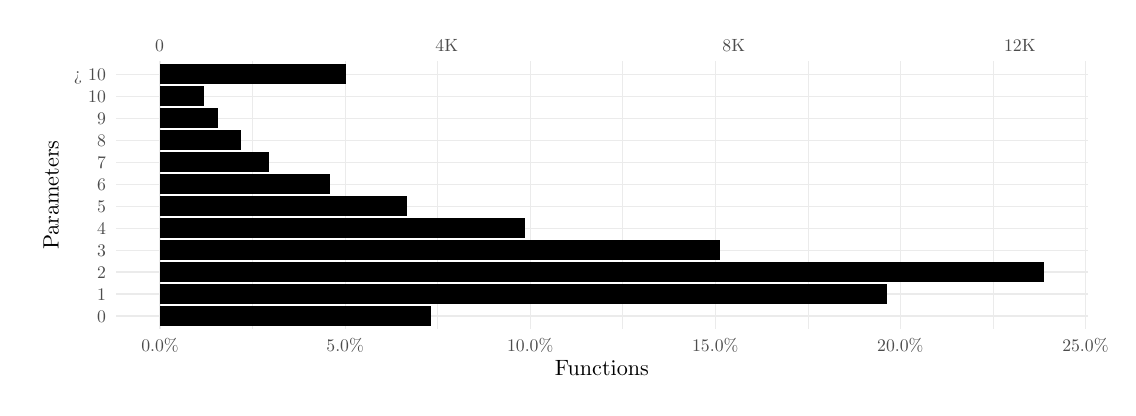
\begin{tikzpicture}[x=1pt,y=1pt]
\definecolor{fillColor}{RGB}{255,255,255}
\path[use as bounding box,fill=fillColor,fill opacity=0.00] (0,0) rectangle (390.26,130.09);
\begin{scope}
\path[clip] ( 31.86, 21.16) rectangle (383.14,117.99);
\definecolor{drawColor}{gray}{0.92}

\path[draw=drawColor,line width= 0.2pt,line join=round] ( 81.27, 21.16) --
	( 81.27,117.99);

\path[draw=drawColor,line width= 0.2pt,line join=round] (148.15, 21.16) --
	(148.15,117.99);

\path[draw=drawColor,line width= 0.2pt,line join=round] (215.02, 21.16) --
	(215.02,117.99);

\path[draw=drawColor,line width= 0.2pt,line join=round] (281.90, 21.16) --
	(281.90,117.99);

\path[draw=drawColor,line width= 0.2pt,line join=round] (348.77, 21.16) --
	(348.77,117.99);

\path[draw=drawColor,line width= 0.4pt,line join=round] ( 31.86, 25.92) --
	(383.14, 25.92);

\path[draw=drawColor,line width= 0.4pt,line join=round] ( 31.86, 33.86) --
	(383.14, 33.86);

\path[draw=drawColor,line width= 0.4pt,line join=round] ( 31.86, 41.80) --
	(383.14, 41.80);

\path[draw=drawColor,line width= 0.4pt,line join=round] ( 31.86, 49.73) --
	(383.14, 49.73);

\path[draw=drawColor,line width= 0.4pt,line join=round] ( 31.86, 57.67) --
	(383.14, 57.67);

\path[draw=drawColor,line width= 0.4pt,line join=round] ( 31.86, 65.61) --
	(383.14, 65.61);

\path[draw=drawColor,line width= 0.4pt,line join=round] ( 31.86, 73.54) --
	(383.14, 73.54);

\path[draw=drawColor,line width= 0.4pt,line join=round] ( 31.86, 81.48) --
	(383.14, 81.48);

\path[draw=drawColor,line width= 0.4pt,line join=round] ( 31.86, 89.42) --
	(383.14, 89.42);

\path[draw=drawColor,line width= 0.4pt,line join=round] ( 31.86, 97.35) --
	(383.14, 97.35);

\path[draw=drawColor,line width= 0.4pt,line join=round] ( 31.86,105.29) --
	(383.14,105.29);

\path[draw=drawColor,line width= 0.4pt,line join=round] ( 31.86,113.23) --
	(383.14,113.23);

\path[draw=drawColor,line width= 0.4pt,line join=round] ( 47.83, 21.16) --
	( 47.83,117.99);

\path[draw=drawColor,line width= 0.4pt,line join=round] (114.71, 21.16) --
	(114.71,117.99);

\path[draw=drawColor,line width= 0.4pt,line join=round] (181.58, 21.16) --
	(181.58,117.99);

\path[draw=drawColor,line width= 0.4pt,line join=round] (248.46, 21.16) --
	(248.46,117.99);

\path[draw=drawColor,line width= 0.4pt,line join=round] (315.34, 21.16) --
	(315.34,117.99);

\path[draw=drawColor,line width= 0.4pt,line join=round] (382.21, 21.16) --
	(382.21,117.99);
\definecolor{fillColor}{RGB}{0,0,0}

\path[fill=fillColor] ( 47.83,109.66) rectangle (115.04,116.80);

\path[fill=fillColor] ( 47.83, 22.35) rectangle (145.68, 29.50);

\path[fill=fillColor] ( 47.83, 30.29) rectangle (310.59, 37.43);

\path[fill=fillColor] ( 47.83,101.72) rectangle ( 63.63,108.86);

\path[fill=fillColor] ( 47.83, 38.23) rectangle (367.18, 45.37);

\path[fill=fillColor] ( 47.83, 46.16) rectangle (250.08, 53.31);

\path[fill=fillColor] ( 47.83, 54.10) rectangle (179.66, 61.24);

\path[fill=fillColor] ( 47.83, 62.04) rectangle (137.11, 69.18);

\path[fill=fillColor] ( 47.83, 69.97) rectangle (109.42, 77.12);

\path[fill=fillColor] ( 47.83, 77.91) rectangle ( 87.10, 85.05);

\path[fill=fillColor] ( 47.83, 85.85) rectangle ( 77.25, 92.99);

\path[fill=fillColor] ( 47.83, 93.78) rectangle ( 68.76,100.93);
\end{scope}
\begin{scope}
\path[clip] (  0.00,  0.00) rectangle (390.26,130.09);
\definecolor{drawColor}{gray}{0.30}

\node[text=drawColor,anchor=base,inner sep=0pt, outer sep=0pt, scale=  0.64] at ( 47.69,121.59) {0};

\node[text=drawColor,anchor=base,inner sep=0pt, outer sep=0pt, scale=  0.64] at (151.42,121.59) {4K};

\node[text=drawColor,anchor=base,inner sep=0pt, outer sep=0pt, scale=  0.64] at (255.15,121.59) {8K};

\node[text=drawColor,anchor=base,inner sep=0pt, outer sep=0pt, scale=  0.64] at (358.53,121.59) {12K};
\end{scope}
\begin{scope}
\path[clip] (  0.00,  0.00) rectangle (390.26,130.09);
\definecolor{drawColor}{gray}{0.30}

\node[text=drawColor,anchor=base east,inner sep=0pt, outer sep=0pt, scale=  0.64] at ( 28.26, 23.72) {0};

\node[text=drawColor,anchor=base east,inner sep=0pt, outer sep=0pt, scale=  0.64] at ( 28.26, 31.66) {1};

\node[text=drawColor,anchor=base east,inner sep=0pt, outer sep=0pt, scale=  0.64] at ( 28.26, 39.59) {2};

\node[text=drawColor,anchor=base east,inner sep=0pt, outer sep=0pt, scale=  0.64] at ( 28.26, 47.53) {3};

\node[text=drawColor,anchor=base east,inner sep=0pt, outer sep=0pt, scale=  0.64] at ( 28.26, 55.47) {4};

\node[text=drawColor,anchor=base east,inner sep=0pt, outer sep=0pt, scale=  0.64] at ( 28.26, 63.40) {5};

\node[text=drawColor,anchor=base east,inner sep=0pt, outer sep=0pt, scale=  0.64] at ( 28.26, 71.34) {6};

\node[text=drawColor,anchor=base east,inner sep=0pt, outer sep=0pt, scale=  0.64] at ( 28.26, 79.28) {7};

\node[text=drawColor,anchor=base east,inner sep=0pt, outer sep=0pt, scale=  0.64] at ( 28.26, 87.21) {8};

\node[text=drawColor,anchor=base east,inner sep=0pt, outer sep=0pt, scale=  0.64] at ( 28.26, 95.15) {9};

\node[text=drawColor,anchor=base east,inner sep=0pt, outer sep=0pt, scale=  0.64] at ( 28.26,103.09) {10};

\node[text=drawColor,anchor=base east,inner sep=0pt, outer sep=0pt, scale=  0.64] at ( 28.26,111.02) {> 10};
\end{scope}
\begin{scope}
\path[clip] (  0.00,  0.00) rectangle (390.26,130.09);
\definecolor{drawColor}{gray}{0.30}

\node[text=drawColor,anchor=base,inner sep=0pt, outer sep=0pt, scale=  0.64] at ( 47.83, 13.15) {0.0{\%}};

\node[text=drawColor,anchor=base,inner sep=0pt, outer sep=0pt, scale=  0.64] at (114.71, 13.15) {5.0{\%}};

\node[text=drawColor,anchor=base,inner sep=0pt, outer sep=0pt, scale=  0.64] at (181.58, 13.15) {10.0{\%}};

\node[text=drawColor,anchor=base,inner sep=0pt, outer sep=0pt, scale=  0.64] at (248.46, 13.15) {15.0{\%}};

\node[text=drawColor,anchor=base,inner sep=0pt, outer sep=0pt, scale=  0.64] at (315.34, 13.15) {20.0{\%}};

\node[text=drawColor,anchor=base,inner sep=0pt, outer sep=0pt, scale=  0.64] at (382.21, 13.15) {25.0{\%}};
\end{scope}
\begin{scope}
\path[clip] (  0.00,  0.00) rectangle (390.26,130.09);
\definecolor{drawColor}{RGB}{0,0,0}

\node[text=drawColor,anchor=base,inner sep=0pt, outer sep=0pt, scale=  0.80] at (207.50,  4.40) {Functions};
\end{scope}
\begin{scope}
\path[clip] (  0.00,  0.00) rectangle (390.26,130.09);
\definecolor{drawColor}{RGB}{0,0,0}

\node[text=drawColor,rotate= 90.00,anchor=base,inner sep=0pt, outer sep=0pt, scale=  0.80] at ( 11.20, 69.58) {Parameters};
\end{scope}
\end{tikzpicture}

  \caption{Parameter Distribution}
  \label{fig:paramDist}
\end{figure}

7.3\% functions have 0 parameters, 19.6\% have 1, and
5.0\% have over 10. There are 15 functions with over 50 parameters that come
from 10 packages. \emph{ComplexHeatmap::pheatmap} (51),
\emph{network::plot.network.default} (52), \emph{rpart.plot::get.layout} (53),
\emph{sna::gplot} (54), \emph{Hmisc::latex.default} (55),
\emph{VennDiagram::draw.quintuple.venn} (57) \emph{pROC::plot.roc.roc} (58),
\emph{rpart.plot::draw.node.numbers} (60), \emph{gplots::heatmap.2} (63),
\emph{Hmisc::event.chart} (66), \emph{ComplexHeatmap::Heatmap} (83),
\emph{ggplot2::theme} (95), \emph{ergm::control.ergm} (117),
\emph{rpart.plot::prp} (119), and
\emph{rpart.plot::check.if.dot.arg.supported.by.rpart.rules} (122) with the
highest number of parameters.

\section{Evaluation}

\subsection{Strictness}

\begin{table}[!h]
  \vspace{-3mm}
  \small
  \caption{Strictness Distribution} \label{table:strictdist}
  \centering
  \begin{tabular}{l|cccr|lr|lr}
    &\bf Unevaluted & \bf Side-Effecting & \bf Reflective & \multicolumn{2}{c}{\textbf{Parameters}} & \multicolumn{2}{c}{\textbf{Functions}}& \bf Packages\\
    \hline
    0&\xmark{}&\xmark{}&\xmark{}&128305&65.25\%&44377&85.93\%&489\\
    1&\xmark{}&\xmark{}&\cmark{}&134&0.07\%&124&0.24\%&47\\
    2&\xmark{}&\cmark{}&\xmark{}&7871&4\%&5805&11.24\%&399\\
    3&\xmark{}&\cmark{}&\cmark{}&408&0.21\%&385&0.75\%&93\\
    4&\cmark{}&\xmark{}&\xmark{}&27050&13.76\%&11333&21.95\%&453\\
    5&\cmark{}&\xmark{}&\cmark{}&13&0.01\%&12&0.02\%&11\\
    6&\cmark{}&\cmark{}&\xmark{}&1213&0.62\%&813&1.57\%&199\\
    7&\cmark{}&\cmark{}&\cmark{}&25&0.01\%&24&0.05\%&15\\
    \hline
  \end{tabular}
\end{table}

\subsection{Robustness}

\subsection{Performance}

\section{Discussion}



\section{Migration Strategy}
- py2to3 does not do a good job
- hack has a simple migration tool
- scala 2 to 3 has migration tools

- If we have signatures for every test on CRAN.
- 


%%\section*{Acknowledgments}
%% TODO: Thank Flip
\bibliography{bib/jv, bib/aviral}

\end{document}
